\documentclass[10pt]{beamer}

\usetheme{metropolis}

\usepackage[export]{adjustbox}
\usepackage{array}
\usepackage{etoolbox}
\usepackage{graphicx}
\usepackage{hyperref}
\usepackage{listings}
\usepackage{pgfplots}
\usepackage{pgfplotstable}
\usepackage{tikz}
\usepackage{xcolor}

\usepgfplotslibrary{fillbetween}
\usepgfplotslibrary{statistics}

\usetikzlibrary{calc}
\usetikzlibrary{patterns}

\hypersetup{
    colorlinks=true,
    linkcolor=white,
    urlcolor=blue!80
}

\definecolor{uiored}{HTML}{DD0000}
\definecolor{uiolightred}{HTML}{FB6666}
\definecolor{uioredtone}{HTML}{FEE0E0}
\definecolor{uioblue}{HTML}{3E31D6}
\definecolor{uiolightblue}{HTML}{86A4F7}
\definecolor{uioblueone}{HTML}{E6ECFF}
\definecolor{uiogreen}{HTML}{2EC483}
\definecolor{uiolightgreen}{HTML}{6CE1AB}
\definecolor{uiogreentone}{HTML}{CEFFDF}
\definecolor{uioorange}{HTML}{FEA11B}
\definecolor{uiolightorange}{HTML}{FDCB87}
\definecolor{uioorangetone}{HTML}{FFE8D4}
\definecolor{uioyellow}{HTML}{FFFEA7}
\definecolor{uiogray}{HTML}{B2B3B7}

\colorlet{mainbackground}{uiored}

\setbeamercolor{frametitle}{bg=mainbackground, fg=white}
\setbeamercolor{title separator}{fg=mainbackground}
\setbeamercolor{progress bar in section page}{fg=white, bg=uiogray}

\def\logowidth{4cm}

\makeatletter
\setbeamertemplate{section page}
{
  \begingroup

    \vspace{4.3cm}
    {\usebeamercolor[fg]{section title}\usebeamerfont{section title}\insertsectionhead}\\[-1ex]
    {\centering\color{white}\rule{\linewidth}{1pt}\par} % the horizontal line

    \vspace*{3.1cm}
    \begin{center}
        
\includegraphics[width=\logowidth,valign=c]{data/uio_logo_full_white.png} % Adjust width and path to your logo as needed
    \end{center}

  \endgroup
}
\makeatother

\AtBeginSection{
  {
    \setbeamercolor{background canvas}{bg=uiored}
    \setbeamercolor{section title}{fg=white}
    \frame[plain,c,noframenumbering]{\sectionpage}
    \setbeamercolor{background canvas}{bg=black!2}
  }
}



\setbeamertemplate{footline}{
    \ifnum\insertframenumber=1
        % Title page, no footer
    \else
        \begin{tikzpicture}[remember picture,overlay]
            \fill[mainbackground] (current page.south west) rectangle ([yshift=0.45cm]current page.south east); % Draw filled rectangle

            % Logo
            \node[anchor=west, yshift=0.225cm] at (current page.south west) {
\includegraphics[height=1.2cm]{data/uio_logo_white.png}};

            % Title and subtitle
            \node[align=center, yshift=0.225cm] at (current page.south) {\textcolor{white}{\textbf{\inserttitle}}\\[0.05cm]\textcolor{white}{\insertsubtitle}};

            % Page number
            \node[anchor=east, yshift=0.225cm, xshift=-0.2cm, align=right] at (current page.south east) {\textcolor{white}{\insertframenumber/\inserttotalframenumber}};
        \end{tikzpicture}
    \fi
}

\subtitle{The role of neuroimaging beyond T1-weighted MRI in the diagnosis and prediction of neuropsychiatric disorders}
\author{Esten H. Leonardsen}
\date{26.10.23}

\definecolor{color1}{HTML}{f94144}
\definecolor{color2}{HTML}{f3722c}
\definecolor{color3}{HTML}{f8961e}
\definecolor{color4}{HTML}{f9c74f}
\definecolor{color5}{HTML}{90be6d}
\definecolor{color6}{HTML}{43aa8b}
\definecolor{color7}{HTML}{577590}

\titlegraphic{
	\centering
	\vspace{7.7cm}
	
\includegraphics[width=\logowidth]{data/uio_logo_full.png}
}

\begin{document}
	% \begin{frame}
	%  	\titlepage
	% \end{frame}

    % \begin{frame}{Overview}
    %     \begin{enumerate}
    %         \item Background: Defining the scope of the lecture.
    %         \item State-of-the-art: How is neuroimaging beyond T1-weighted MRI currently being used with respect to neuropsychiatric disorders.
    %         \item The future: Challenges and opportunities in using neuroimaging for predicting neuropsychiatric disorders moving forward.
    %     \end{enumerate}
    % \end{frame}

    % \begin{frame}[t]{Background}
    %     \centering
    %     \begin{tikzpicture}
    %         \colorlet{hiddencolour}{black!20}

    %         \def\labelsize{\scriptsize}

    %         \node[] at (0, 0) {};
    %         \node[draw=black] at (-5, 0) {};
    %         \node[draw=black] at (5, -7) {};
    %         \onslide<1>{
    %             \node[align=center] at (0, -0.5) {
    %                 The role of neuroimaging beyond T1-weighted MRI in the\\diagnosis and prediction of neuropsychiatric disorders
    %             };
    %         }
    %         \only<2-6>{
    %             \node[align=center] at (0, -0.5) {
    %                 \textcolor{hiddencolour}{The role of }neuroimaging \textcolor{hiddencolour}{beyond T1-weighted MRI in the}\\\textcolor{hiddencolour}{diagnosis and prediction of neuropsychiatric disorders}
    %             };
    %             \onslide<3->{
    %                 \node[inner sep=0pt, label=below:{\labelsize{Bert from FreeSurfer 7.3}}] at (-3, -4) {
    %                     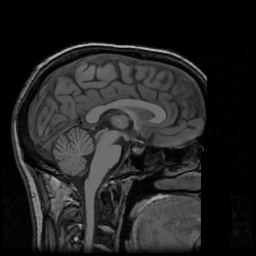
\includegraphics[width=3cm]{data/bert_sagittal.png}
    %                 };
    %             }
    %             \onslide<4->{
    %                 \node[label=below:{\labelsize{Sample from the MNE library}}] at (1.5, -2.5) {
    %                     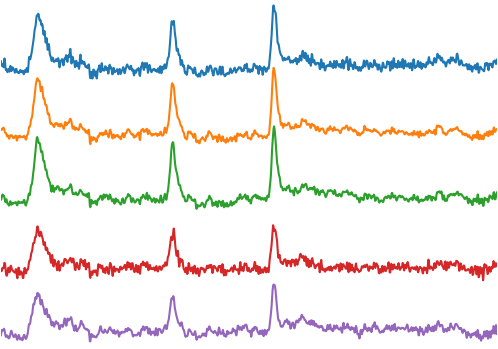
\includegraphics[width=3.75cm]{data/eeg.png}
    %                 };
    %             }
    %             \onslide<5->{
    %                 %https://www.ncbi.nlm.nih.gov/pmc/articles/PMC4980915/
    %                 \node[label=below:{\labelsize{Sample from Tremlay et al., 2016}}] at (0.7, -5.1) {
    %                     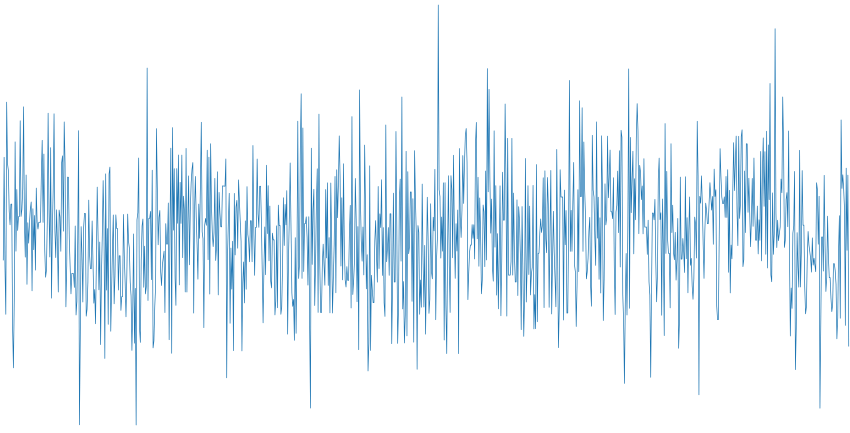
\includegraphics[width=3cm]{data/patch_clamp.png}
    %                 };
    %                 \node[font=\tiny, align=center] at (0, -7.5) {
    %                     Tremblay, R., Lee, S., \& Rudy, B. (2016). GABAergic interneurons in the neocortex: from cellular properties to circuits. Neuron,\\91(2), 260-292
    %                 };
    %             }
    %             \onslide<6->{
    %                 \node[label=below:{\labelsize{Meta Quest Pro}}] at (3.75, -6.1) {
    %                     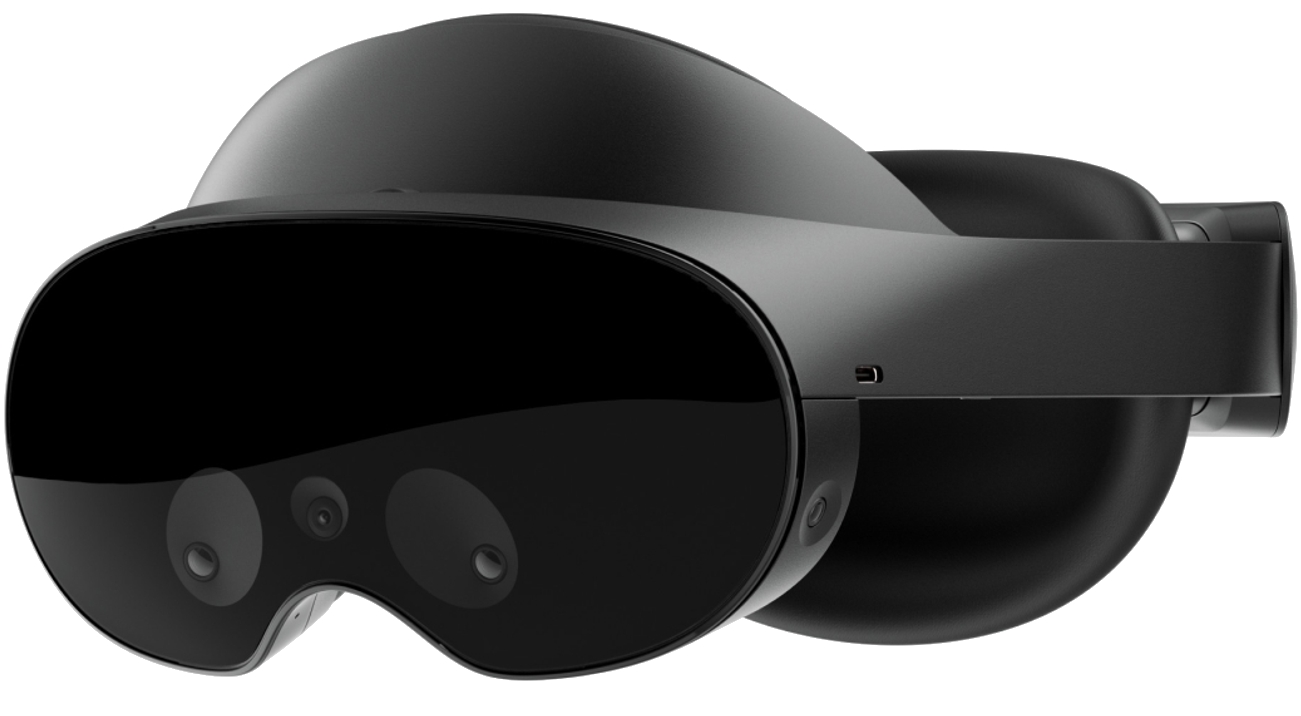
\includegraphics[width=2cm]{data/meta_quest.png}
    %                 };
    %             }
    %         }
    %         \only<7-12>{
    %             \node[align=center] at (0, -0.5) {
    %                 \textcolor{hiddencolour}{The role of neuroimaging beyond }T1-weighted MRI \textcolor{hiddencolour}{in the}\\\textcolor{hiddencolour}{diagnosis and prediction of neuropsychiatric disorders}
    %             };
    %             \onslide<8->{
    %                 \node[inner sep=0pt, label=below:{\labelsize{Bert from FreeSurfer 7.3}}] at (-3, -3.5) {
    %                     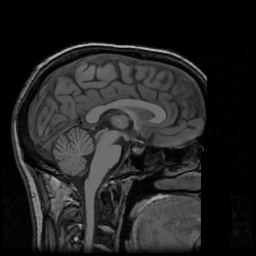
\includegraphics[width=3cm]{data/bert_sagittal.png}
    %                 };
    %             }
    %             \onslide<10->{
    %                 %https://doi.org/10.1016/j.neuroimage.2016.02.079
    %                 \node[inner sep=0pt, draw=black, inner sep=0pt, label=below:{\labelsize{Arbabshirani et al., 2017}}] at (1, -2.5) {
    %                     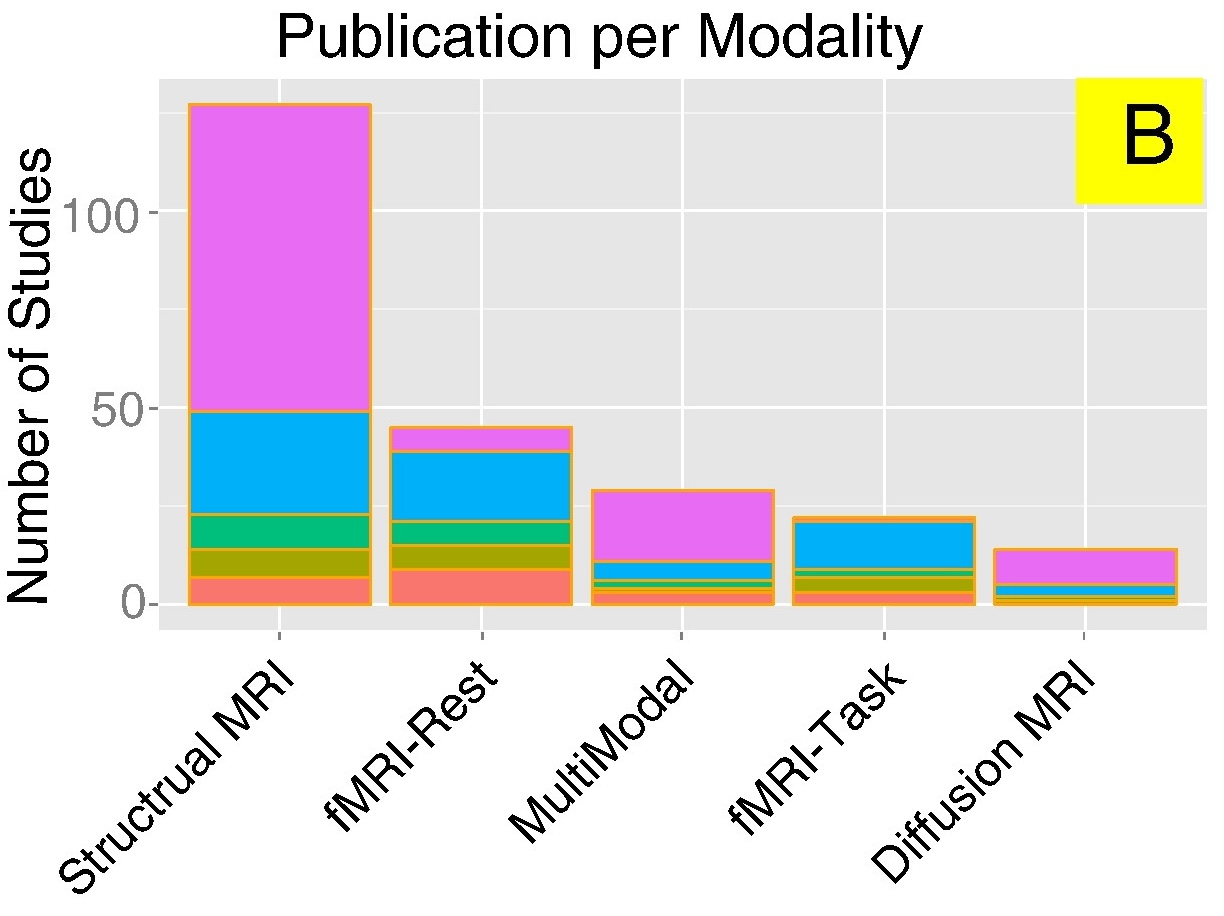
\includegraphics[width=3.5cm]{data/arbabshirani_modalities.jpg}
    %                 };
    %                 \only<10>{
    %                     \node[font=\tiny,align=center, inner sep=1pt] (arbabshirani-citation) at (0, -7.7) {
    %                         Arbabshirani, M. R., Plis, S., Sui, J., \& Calhoun, V. D. (2017). Single subject prediction of brain disorders inneuroimaging: Promises\\and pitfalls. Neuroimage, 145, 137-165
    %                     };
    %                 }
    %             }
    %             \onslide<11->{
    %                 \node[inner sep=0pt, draw=black, inner sep=0pt, label=below:{\labelsize{Ebrahimighahnavieh et al., 2020}}] at (1.3, -3.6) {
    %                     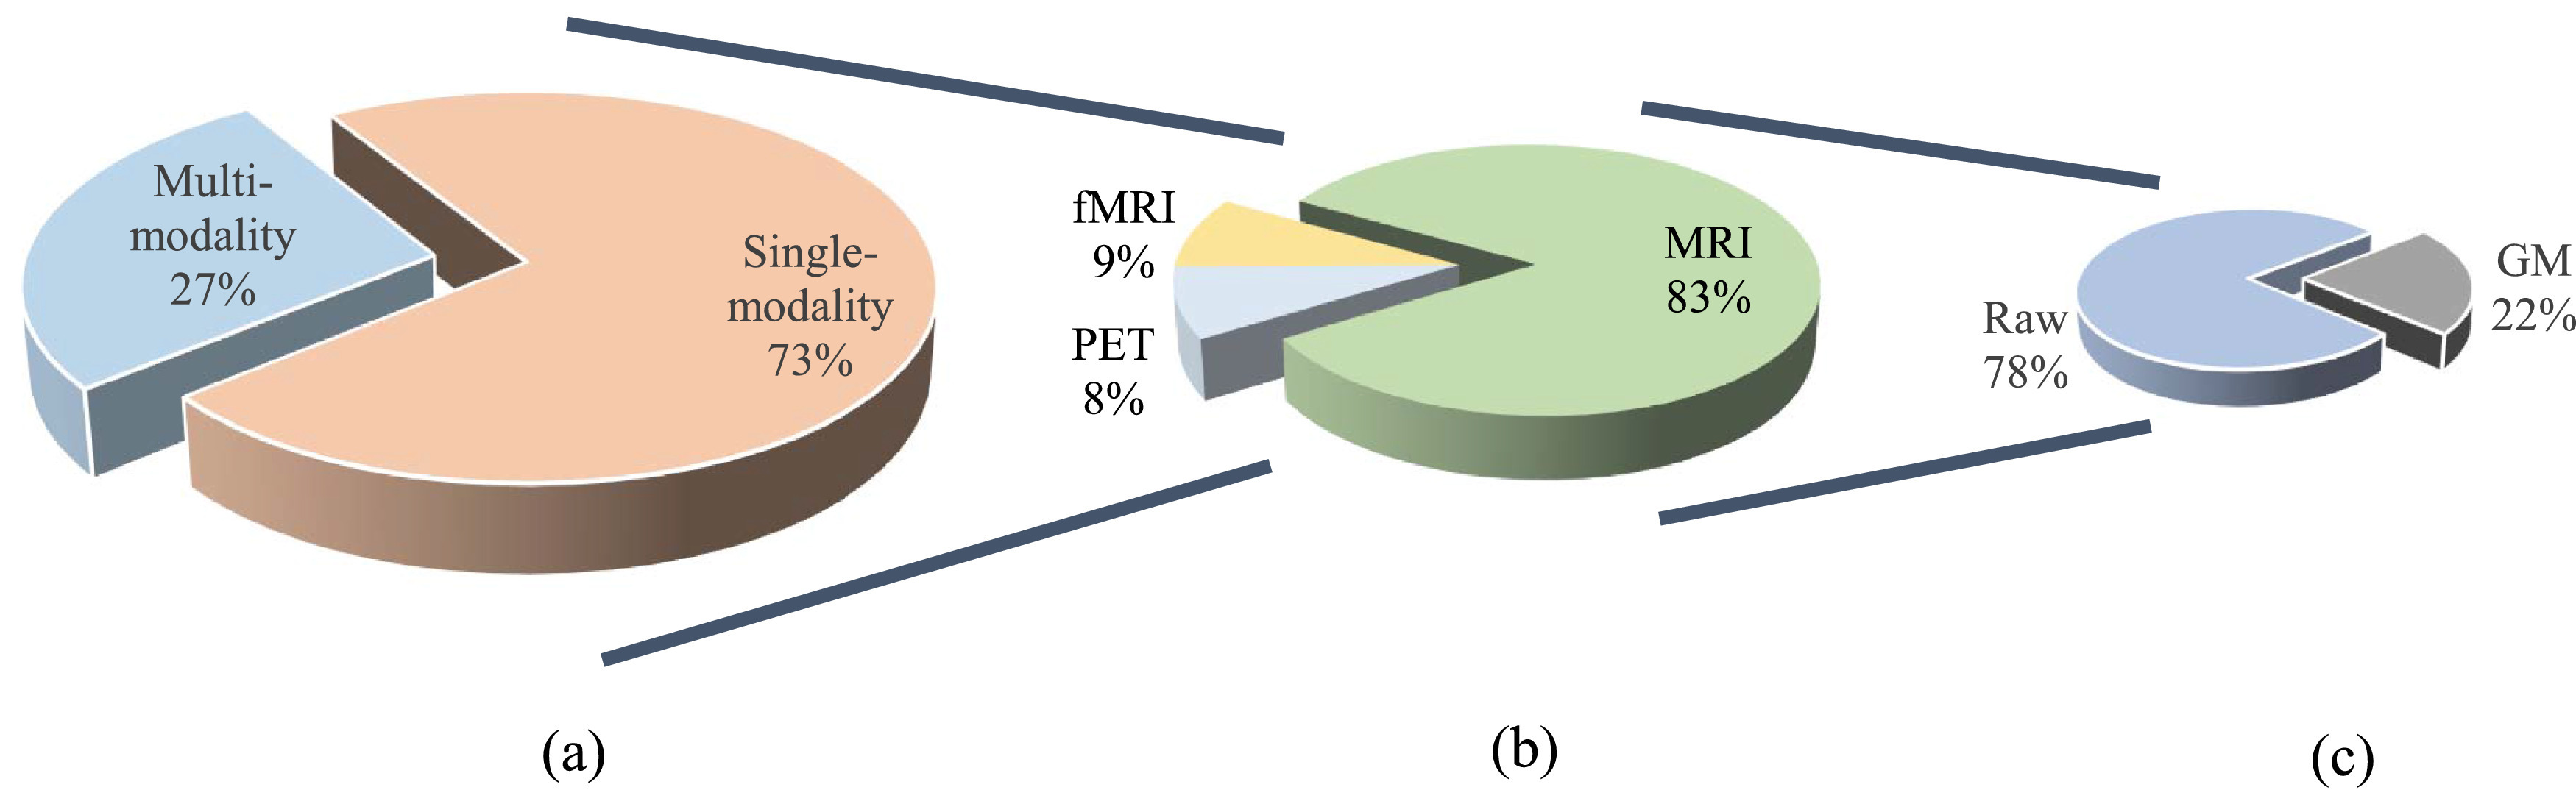
\includegraphics[width=3.7cm]{data/alzheimer_modalities.jpg}
    %                 };
    %                 \only<11>{
    %                     \node[font=\tiny, anchor=south,align=center, inner sep=1pt] (alz-citation) at (0, -7.7) {
    %                         Ebrahimighahnavieh, M. A., Luo, S., \& Chiong, R. (2020). Deep learning to detect Alzheimer's disease from neuroimaging: A\\systematic literature review. Computer methods and programs in biomedicine, 187, 105242
    %                     };
    %                 }
    %             }
    %             \onslide<12->{
    %                 \node[inner sep=0pt, draw=black, inner sep=0pt, label=below:{\labelsize{Quaak et al., 2020}}] at (1.3, -3.5) {
    %                     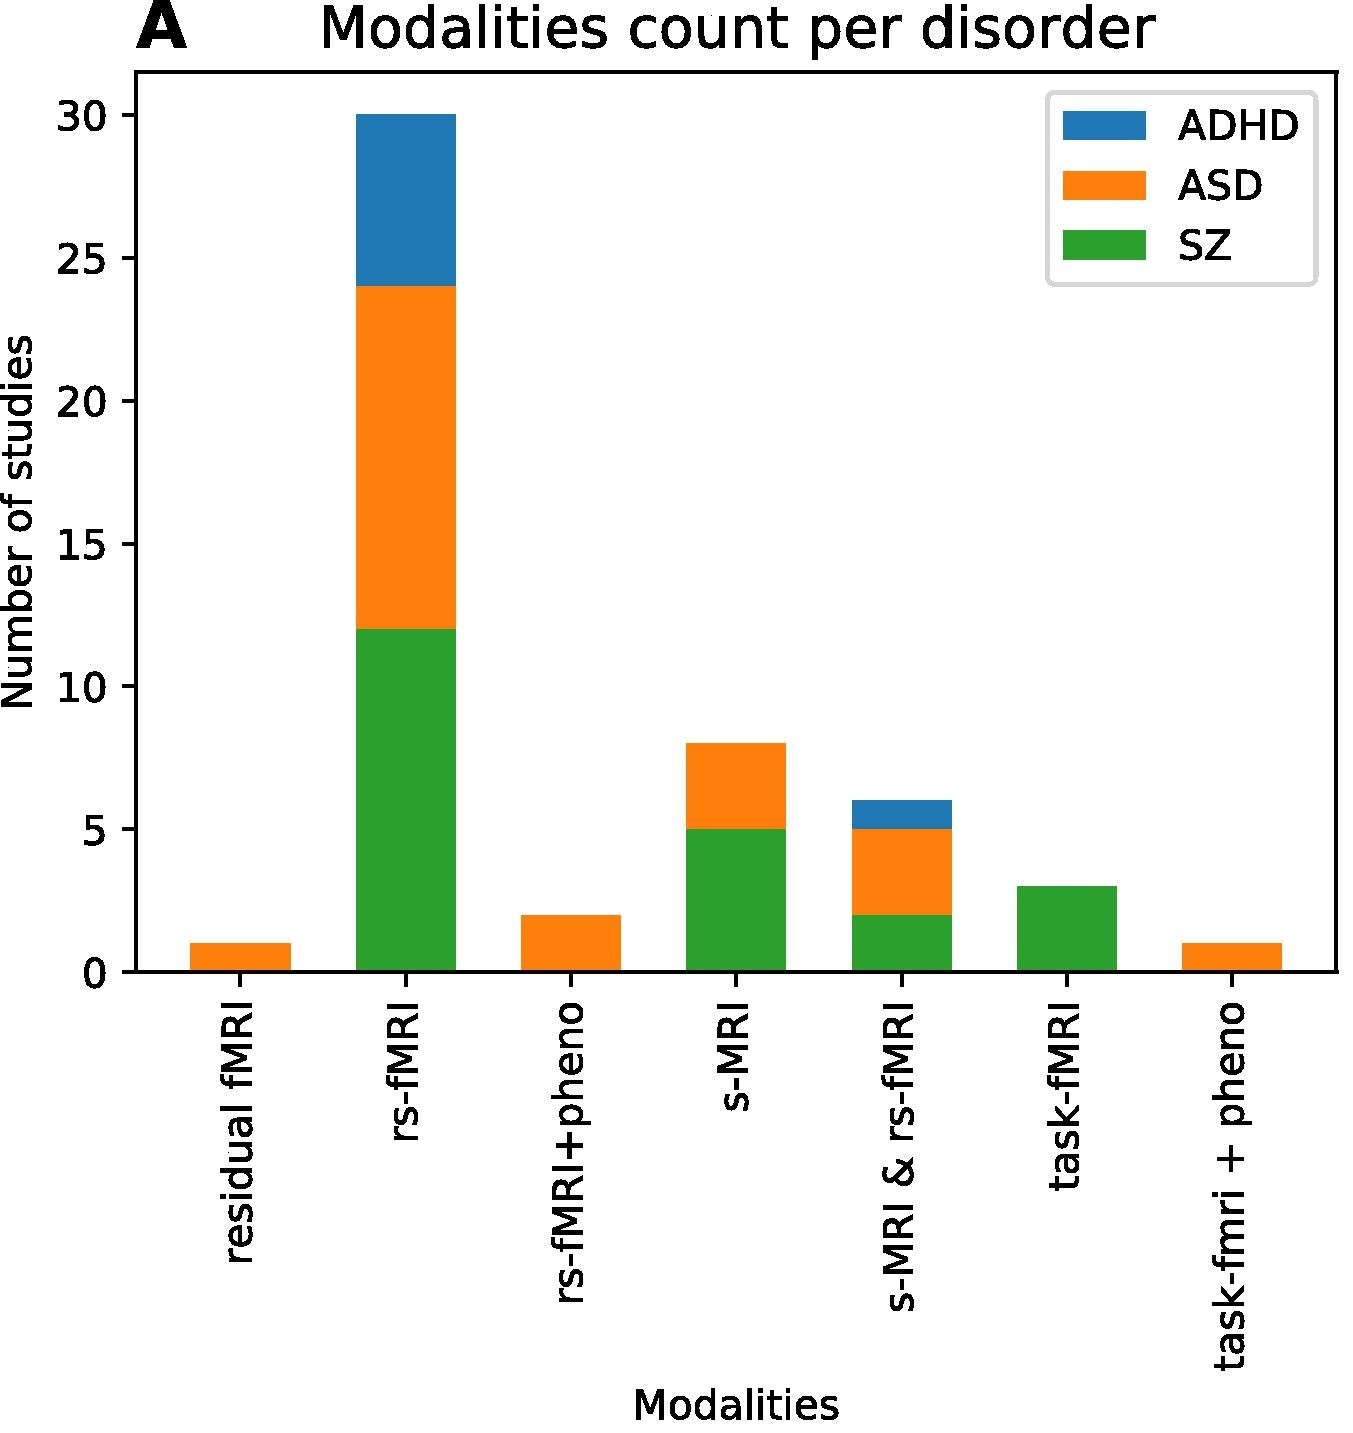
\includegraphics[width=3.6cm]{data/quaak_modalities.jpg}
    %                 };
    %                 \only<12>{
    %                     \node[font=\tiny, anchor=south,align=center, inner sep=1pt] (psych-citation) at (0, -7.7) {
    %                         Quaak, M., van de Mortel, L., Thomas, R. M., \& van Wingen, G. (2021). Deep learning applications for the classification of psychiatric\\disorders using neuroimaging data: systematic review and meta-analysis. NeuroImage: Clinical, 30, 102584
    %                     };
    %                 }
    %             }
    %         }
    %         \only<13-17>{
    %             \def\nodefont{\footnotesize}
    %             \node[align=center] at (0, -0.5) {
    %                 \textcolor{hiddencolour}{The role of neuroimaging beyond T1-weighted MRI in the}\\\textcolor{hiddencolour}{diagnosis and prediction of }neuropsychiatric disorders
    %             };
    %             \onslide<14->{
    %                 \node[align=center, font=\nodefont] at (-2, -2) {
    %                     Alzheimer's disease and other\\causes of dementia
    %                 };
    %                 \node[align=center, font=\nodefont] at (-2.8, -2.8) {
    %                     Multiple Sclerosis
    %                 };
    %                 \node[align=center, font=\nodefont] at (-1.3, -3.2) {
    %                     Parkinson's Disease
    %                 };
    %             }

    %             \onslide<15->{
    %                 \node[align=center, font=\nodefont] at (1.9, -2.2) {
    %                     Bipolar Disorder
    %                 };
    %                 \node[align=center, font=\nodefont] at (1.6, -2.6) {
    %                     Schizophrenia
    %                 };
    %                 \node[align=center, font=\nodefont] at (2.8, -3.3) {
    %                     Depressive disorders
    %                 };
    %             }
    %             \onslide<16->{
    %                 \draw[stealth-stealth] (-4, -4) -- (4, -4);
    %             }
    %             \only<16>{
    %                 \node[anchor=east] at (-4, -4) {
    %                     \small{More}
    %                 };
    %                 \node[anchor=west] at (4, -4) {
    %                     \small{Less}
    %                 };
    %                 \node[anchor=north, font=\small] at (0, -4.1) {
    %                     Knowledge about neuropathological basis
    %                 };
    %             }
    %             \only<17>{
    %                 \node[anchor=east] at (-4, -4) {
    %                     \small{Less}
    %                 };
    %                 \node[anchor=west] at (4, -4) {
    %                     \small{More}
    %                 };
    %                 \node[anchor=north, font=\small] at (0, -4.1) {
    %                     Importance of psychopathology
    %                 };
    %             }
    %         }
    %         \onslide<18->{
    %             \node[align=center] at (0, -0.5) {
    %                 \textcolor{hiddencolour}{The role of neuroimaging beyond T1-weighted MRI in the}\\diagnosis and prediction \textcolor{hiddencolour}{of neuropsychiatric disorders}
    %             };
    %             \only<19>{
    %                 \node[label=below:{\labelsize{Vogel \& Black (2024)}}, inner sep=0pt, draw=black] at (0, -3.5) {
    %                     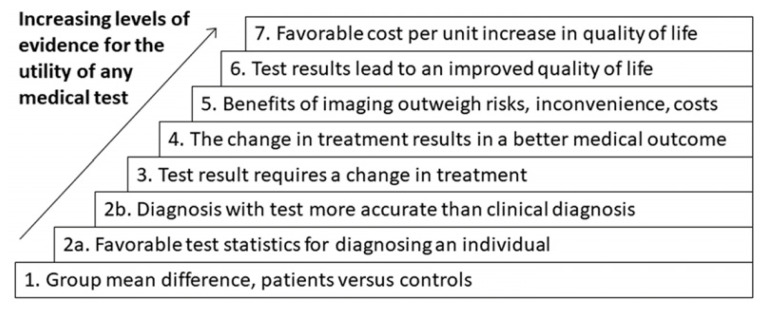
\includegraphics[width=7cm]{data/diagnostic_predictions.jpeg}
    %                 };

    %                 \node[font=\tiny, anchor=south,align=center, inner sep=1pt] (psych-citation) at (0, -7.7) {
    %                     Vogel, A. C., \& Black, K. J. (2024). Brain Imaging in Routine Psychiatric Practice. Missouri Medicine, 121(1), 37
    %                 };

    %             }
    %         }
    %         %     \only<10>{
    %         %         %https://doi.org/10.1016/S2215-0366(21)00395-3
    %         %         \node[inner sep=0pt, draw=black] at (3, -4) {
    %         %             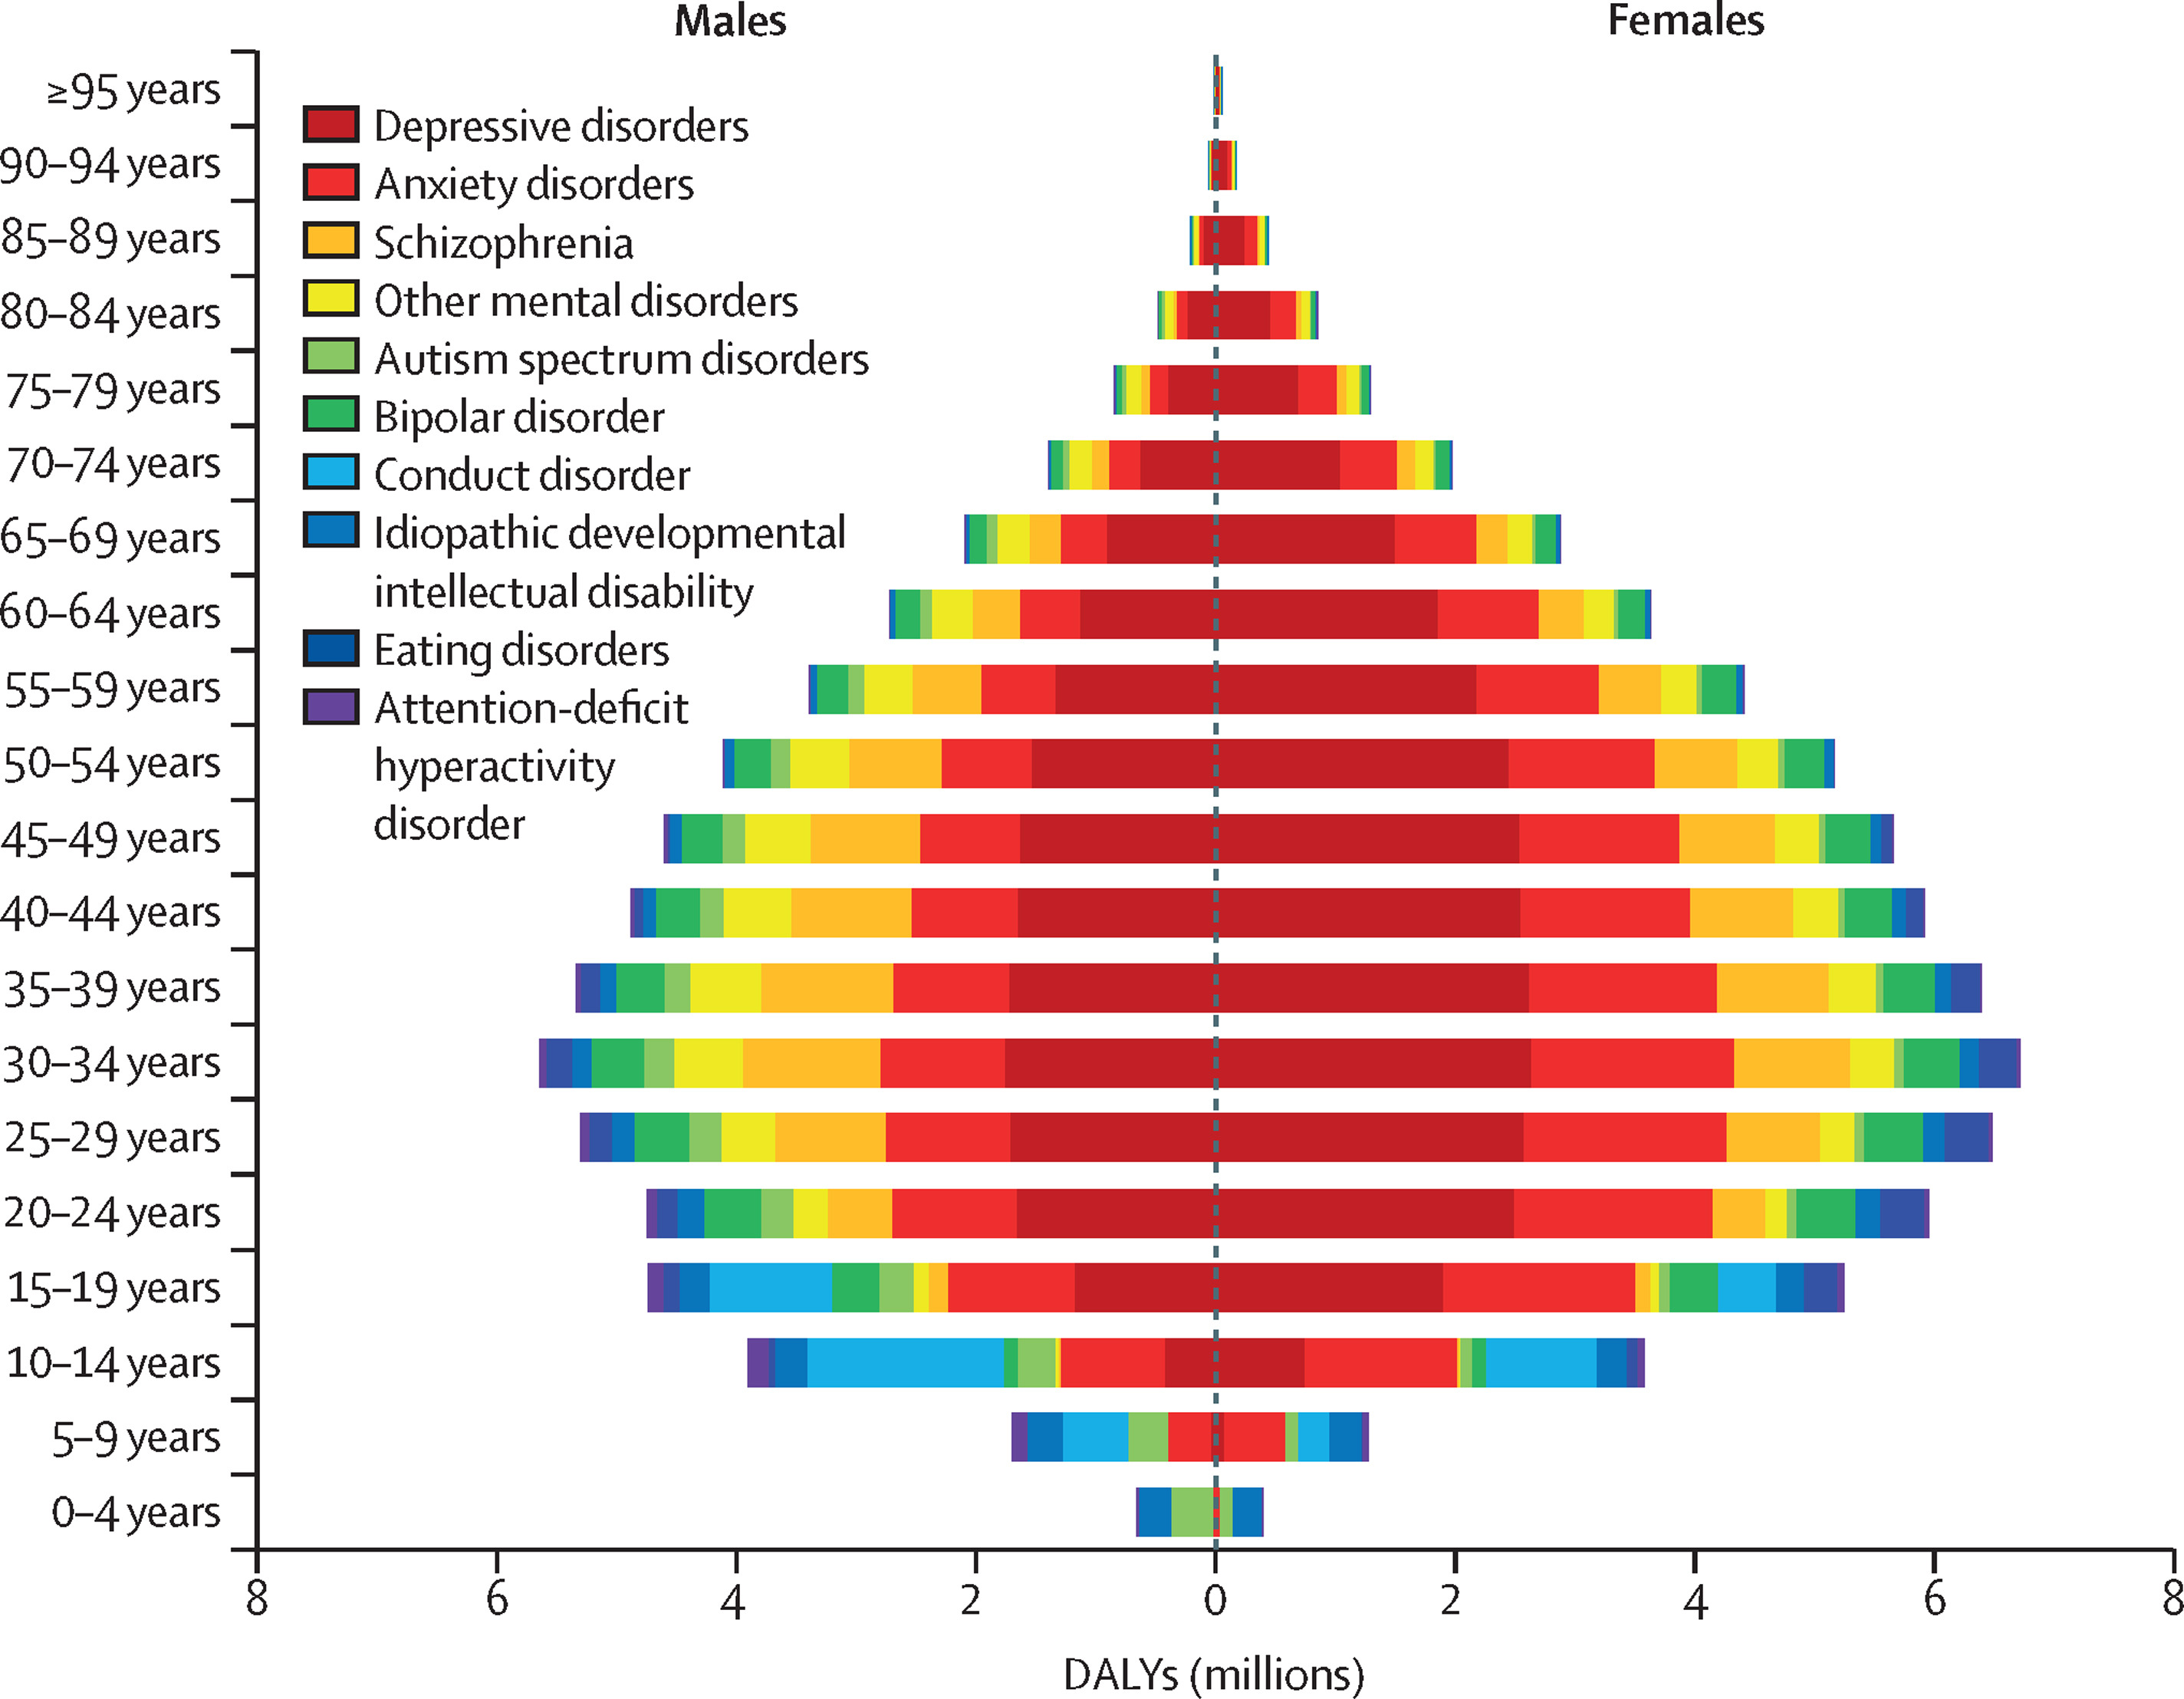
\includegraphics[width=5cm]{data/mental_disorder_dalys.jpeg}
    %         %         };
    %         %     }
    %         % }
    %         % \only<11>{

    %         % }
    %     \end{tikzpicture}
    % \end{frame}
    % \section{The current roles of neuroimaging modalities}

    % \newsavebox{\ttwostudies}
    % \sbox{\ttwostudies}{%
    %     \begin{tikzpicture}
    %         \begin{axis}[
    %             ymin=50,
    %             ymax=100,
    %             xtick={2016, 2018, 2020, 2022},
    %             xticklabels={2016, 2018, 2020, 2022},
    %             xlabel=Year,
    %             ylabel=Accuracy,
    %             width=5cm,
    %             height=5cm,
    %             every tick label/.append style={font=\footnotesize},
    %             xtick pos=bottom,
    %             ytick pos=left,
    %             clip=false,
    %             xmin=2015.5,
    %             xmax=2022.5
    %         ]
    %             \addplot[
    %                 only marks,
    %                 scatter,
    %                 scatter/classes={
    %                     MS={mark=*,color1},
    %                     PD={mark=*,color4}
    %                 },
    %                 scatter src=explicit symbolic,
    %                 visualization depends on={ln(\thisrow{sample}*0.5) \as \perpointmarksize},
    %                 scatter/@pre marker code/.append style={
    %                     /tikz/mark size=\perpointmarksize
    %                 },
    %                 opacity=0.75
    %             ] table [
    %                 x=year,
    %                 y=accuracy,
    %                 col sep=comma,
    %                 meta=diagnosis
    %             ] {data/t2_studies.csv};
    %         \end{axis}
    %     \end{tikzpicture}
    % }

    % \begin{frame}{Other structural MRI modalities (T2, FLAIR)}
    %     \centering
    %     \begin{tikzpicture}
    %         \def\labelsize{\footnotesize}

    %         \node[draw=black] at (0, 0) {};
    %         \node[draw=black] at (10, -7) {};
    %         \onslide<1->{
    %             \node[anchor=west] (t1) at (0, -3.5) {
    %                 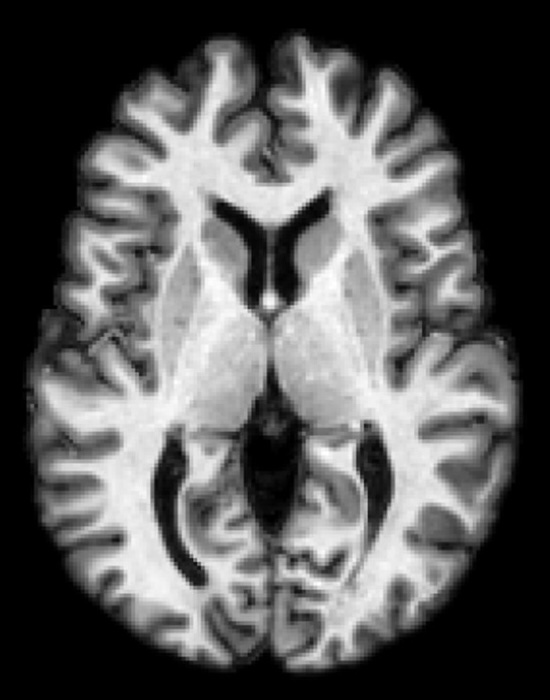
\includegraphics[
    %                     height=1.7cm
    %                 ]{data/t1.jpg}
    %             };
    %             \node[anchor=south, inner sep=0pt] at (t1.north) {\labelsize{T1}};
    %         }
    %         \onslide<2->{
    %             \node[anchor=west] (t2) at ($ (t1.east) - (0.35, 0) $) {
    %                 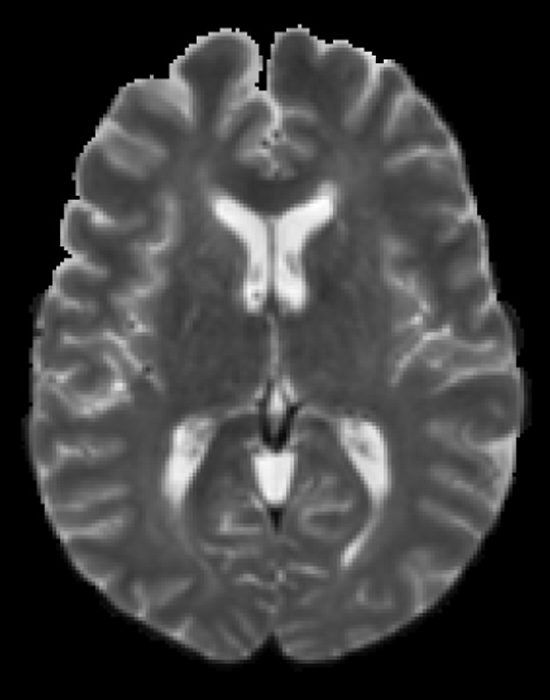
\includegraphics[
    %                     height=1.7cm
    %                 ]{data/t2.jpg}
    %             };
    %             \node[anchor=south, inner sep=0pt] at (t2.north) {\labelsize{T2}};
    %         }
    %         \onslide<3->{
    %             \node[anchor=west] (flair) at ($ (t2.east) - (0.35, 0) $) {
    %                 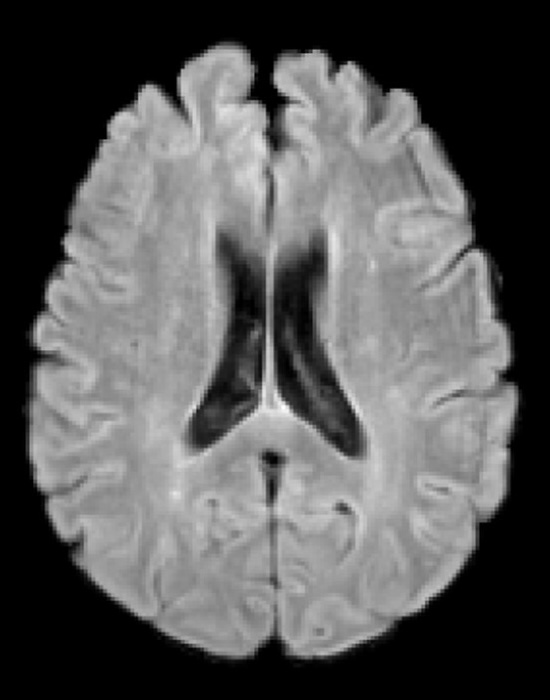
\includegraphics[
    %                     height=1.7cm
    %                 ]{data/flair.jpg}
    %             };
    %             \node[anchor=south, inner sep=0pt] at (flair.north) {\labelsize{FLAIR}};
    %             \node[anchor=north] at ($ (t2.south) - (0, -0.15) $) {\scriptsize{Adapted from Shoeibi et al., 2021}};
    %             \only<3>{
    %                 \node[font=\tiny, anchor=south,align=center, inner sep=1pt] (ms-citation) at (5, -7.5) {
    %                     Shoeibi, A., Khodatars, M., Jafari, M., Moridian, P., Rezaei, M., Alizadehsani, R., ... \& Acharya, U. R. (2021). Applications of deep learning\\techniques for automated multiple sclerosis detection using magnetic resonance imaging: A review. Computers in Biology and\\Medicine, 136, 104697
    %                 };
    %             }
    %         }
    %         \only<4>{
    %             \node[] at (7.6, -3.2) {
    %                 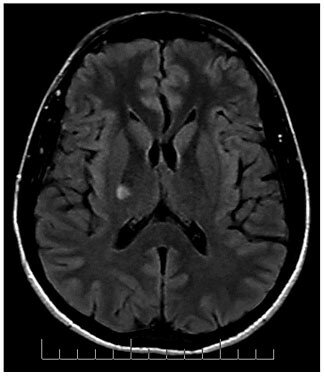
\includegraphics[width=4cm]{data/flair_lesion.jpeg}
    %             };
    %         }
    %         \only<5>{
    %             \node[] at (7.6, -3.2) {
    %                 \usebox{\ttwostudies}
    %             };
    %         };
    %         \only<6>{
    %             \node[label=below:\scriptsize{De Angelis et al., 2019}, inner sep=0pt, draw=black] at (7.6, -3.2) {
    %                 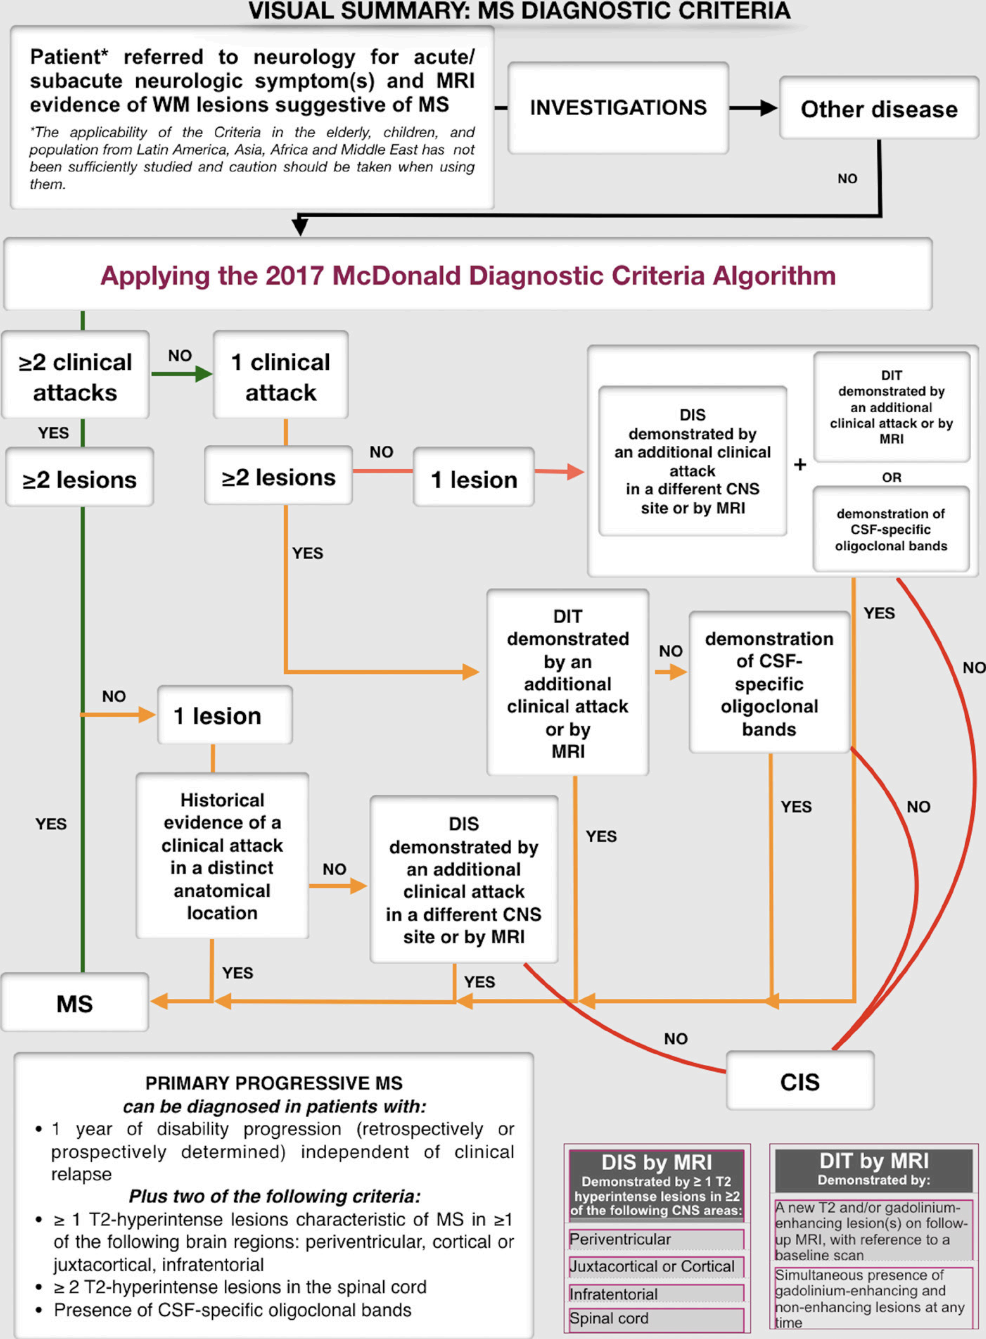
\includegraphics[width=4.5cm]{data/ms_criteria.png}
    %             };
    %             \node[font=\tiny, anchor=south,align=center, inner sep=1pt] (ms-citation) at (5, -7.5) {
    %                 De Angelis, F., Brownlee, W. J., Chard, D. T., \& Trip, S. A. (2019). New MS diagnostic criteria in practice. Practical Neurology, 19(1), 64-67
    %             };
    %         }
    %         \only<7>{
    %             \node[] at (7.6, -3.2) {
    %                 T2 use-case in PD: WML/Motoric problems
    %             };
    %         }
    %         \only<8>{
    %             \node[] at (7.6, -3.2) {
    %                 T2 use-case in dementia: WML/Subtyping
    %             };
    %         }
    %     \end{tikzpicture}
    % \end{frame}

    % \newsavebox{\dmristudies}
    % \sbox{\dmristudies}{%
    %     \begin{tikzpicture}
    %         \begin{axis}[
    %             ymin=50,
    %             ymax=100,
    %             xlabel=Year,
    %             ylabel=Accuracy,
    %             width=5cm,
    %             height=5cm,
    %             every tick label/.append style={font=\footnotesize},
    %             xtick pos=bottom,
    %             ytick pos=left,
    %         ]
    %             \addplot[
    %                 only marks,
    %                 scatter,
    %                 scatter/classes={
    %                     AD={mark=*,color1},
    %                     SCZ={mark=*,color3},
    %                     MDD={mark=*,color5},
    %                     BP={mark=*,color7}
    %                 },
    %                 scatter src=explicit symbolic,
    %                 visualization depends on={ln(\thisrow{sample}*0.5) \as \perpointmarksize},
    %                 scatter/@pre marker code/.append style={
    %                     /tikz/mark size=\perpointmarksize
    %                 },
    %                 opacity=0.75
    %             ] table [
    %                 x=year,
    %                 y=accuracy,
    %                 col sep=comma,
    %                 meta=diagnosis
    %             ] {data/dMRI_studies.csv};
    %         \end{axis}
    %     \end{tikzpicture}
    % }

    % \begin{frame}{Diffusion MRI (DTI?)}
    %     \begin{tikzpicture}
    %         \node[draw=black] at (0, 0) {};
    %         \node[draw=black] at (10, -7) {};

    %         \onslide<1->{
    %             \node[] at (2, -3.5) {
    %                 Explanation of DTI
    %             };
    %         }
    %         \only<2>{
    %             \node[] at (7.6, -3.2) {
    %                 \usebox{\dmristudies}
    %             };
    %         };
    %         \only<3>{
    %             \node[] at (7.6, -3.2) {
    %                 Lack of prediction studies
    %             };
    %         }
    %         \only<4>{
    %             \node[] at (7.6, -3.2) {
    %                 DTI use case 1
    %             };
    %         }
    %         \only<5>{
    %             \node[] at (7.6, -3.2) {
    %                 DTI use case 2
    %             };
    %         }
    %     \end{tikzpicture}
    % \end{frame}

    % \begin{frame}{Molecular imaging (PET/SPECT)}
    %     % https://www.ncbi.nlm.nih.gov/pmc/articles/PMC9181385/#B45-ijms-23-06079
    %     \begin{tikzpicture}
    %         \node[draw=black] at (0, 0) {};
    %         \node[draw=black] at (10, -7) {};

    %         \onslide<1->{
    %             \node[] at (2, -3.5) {
    %                 Explanation of PET
    %             };
    %         }
    %         \only<2>{
    %             \node[] at (7.6, -3.2) {
    %                 PET/SPECT in meta-analysis
    %             };
    %         };
    %         \only<3>{
    %             \node[] at (7.6, -3.2) {
    %                 PET in AD
    %             };
    %         }
    %         \only<4>{
    %             \node[] at (7.6, -3.2) {
    %                 SPECT in PD
    %             };
    %         }
    %         \only<5>{
    %             \node[] at (7.6, -3.2) {
    %                 Mental disorders?
    %             };
    %         }
    %     \end{tikzpicture}
    % \end{frame}

    % \newsavebox{\fmristudies}
    % \sbox{\fmristudies}{%
    %     \begin{tikzpicture}
    %         \begin{axis}[
    %             ymin=50,
    %             ymax=100,
    %             xlabel=Year,
    %             ylabel=Accuracy,
    %             width=5cm,
    %             height=5cm,
    %             every tick label/.append style={font=\footnotesize},
    %             xtick pos=bottom,
    %             ytick pos=left,
    %         ]
    %             \addplot[
    %                 only marks,
    %                 scatter,
    %                 scatter/classes={
    %                     AD={mark=*,color1},
    %                     SCZ={mark=*,color3},
    %                     MDD={mark=*,color5},
    %                     BP={mark=*,color7}
    %                 },
    %                 scatter src=explicit symbolic,
    %                 visualization depends on={ln(\thisrow{sample}*0.5) \as \perpointmarksize},
    %                 scatter/@pre marker code/.append style={
    %                     /tikz/mark size=\perpointmarksize
    %                 },
    %                 opacity=0.75
    %             ] table [
    %                 x=year,
    %                 y=accuracy,
    %                 col sep=comma,
    %                 meta=diagnosis
    %             ] {data/fMRI_studies.csv};
    %         \end{axis}
    %     \end{tikzpicture}
    % }

    % \begin{frame}{Functional Magnetic Resonance Imaging (fMRI)}
    %     \begin{tikzpicture}
    %         \node[draw=black] at (0, 0) {};
    %         \node[draw=black] at (10, -7) {};

    %         \onslide<1->{
    %             \node[] at (2, -3.5) {
    %                 Explanation of fMRI
    %             };
    %         }
    %         \only<2>{
    %             \node[] at (7.6, -3.2) {
    %                 Task vs rest
    %             };
    %         };
    %         \only<3>{
    %             \node[] at (7.6, -3.2) {
    %                 \usebox{\fmristudies}
    %             };
    %         }
    %         \only<4>{
    %             \node[] at (7.6, -3.2) {
    %                 fMRI use-case 1
    %             };
    %         }
    %         \only<5>{
    %             \node[] at (7.6, -3.2) {
    %                 fMRI use-case 2
    %             };
    %         }
    %     \end{tikzpicture}
    % \end{frame}

    % \begin{frame}{Elecrophysiological mapping (EEG/MEG)}
    % \end{frame}

    % \begin{frame}{Alzheimer's disease}
    %     \centering
    %     \begin{itemize}
    %         \item Pathological changes are apparent in a variety of neuroimaging modalities, to a level which can support individual diagnostics.
    %         \item
    %     \end{itemize}
    %     \begin{tikzpicture}
    %         %https://www.ncbi.nlm.nih.gov/pmc/articles/PMC9181385/
    %         \node[inner sep=0pt, draw=black] at (0, 0) {
    %             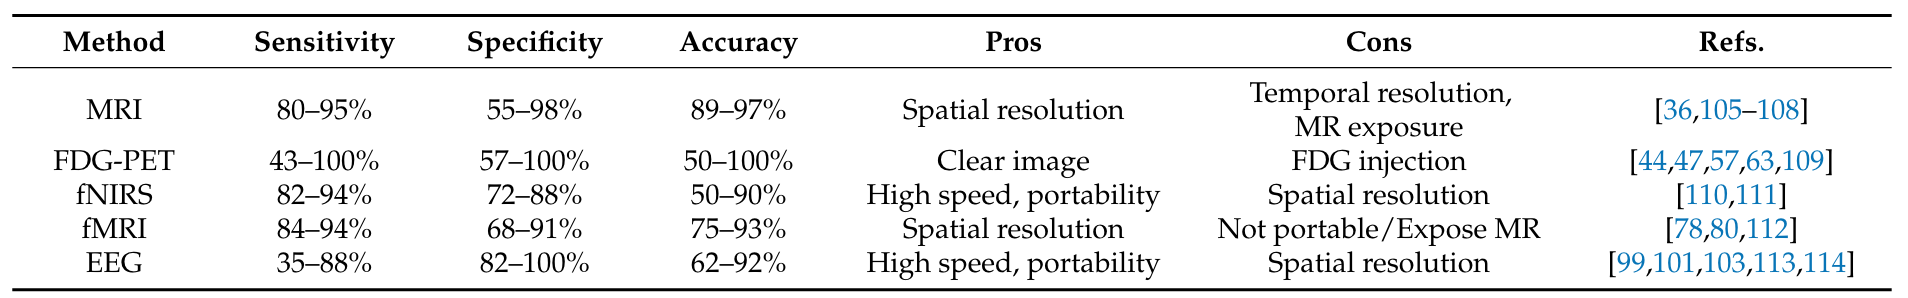
\includegraphics[width=9cm]{data/AD_modalities.png}
    %         };
    %     \end{tikzpicture}
    % \end{frame}
    % \begin{frame}{Multiple sclerosis}
    %     \begin{itemize}
    %         \item Lesions apparent in T2-weighted and FLAIR images are used clinically to support diagnostics.
    %         \item DTI reveals group-wise differences also in apparently healthy white matter.
    %         \item A stereotypical trajectory that has been observed in patients using fMRI is heightened activation up until a point where it is no longer possible to compensate for structural damage, after which the activation generally resides.
    %     \end{itemize}
    % \end{frame}
    % \begin{frame}{Parkinson's disease}
    %     % https://www.ncbi.nlm.nih.gov/pmc/articles/PMC6280219/
    %     % https://link.springer.com/article/10.1007/s12559-023-10175-y
    %     \begin{itemize}
    %         \item DTI has been shown useful for classifying patient subtypes and correlates with motor and cognitive function in PD patients.
    %         \item fMRI has been shown useful for differentiating patient subtypes, supporting the notion of PD subtypes as network models.
    %         \item PET imaging can be used to reveal subtypes
    %     \end{itemize}
    % \end{frame}

    % \begin{frame}{Bipolar disorder}
    %     \begin{tikzpicture}
    %         \only<1>{
    %             % https://pubmed.ncbi.nlm.nih.gov/32108409/
    %             \node[inner sep=0pt, draw=black] at (0, 0) {
    %                 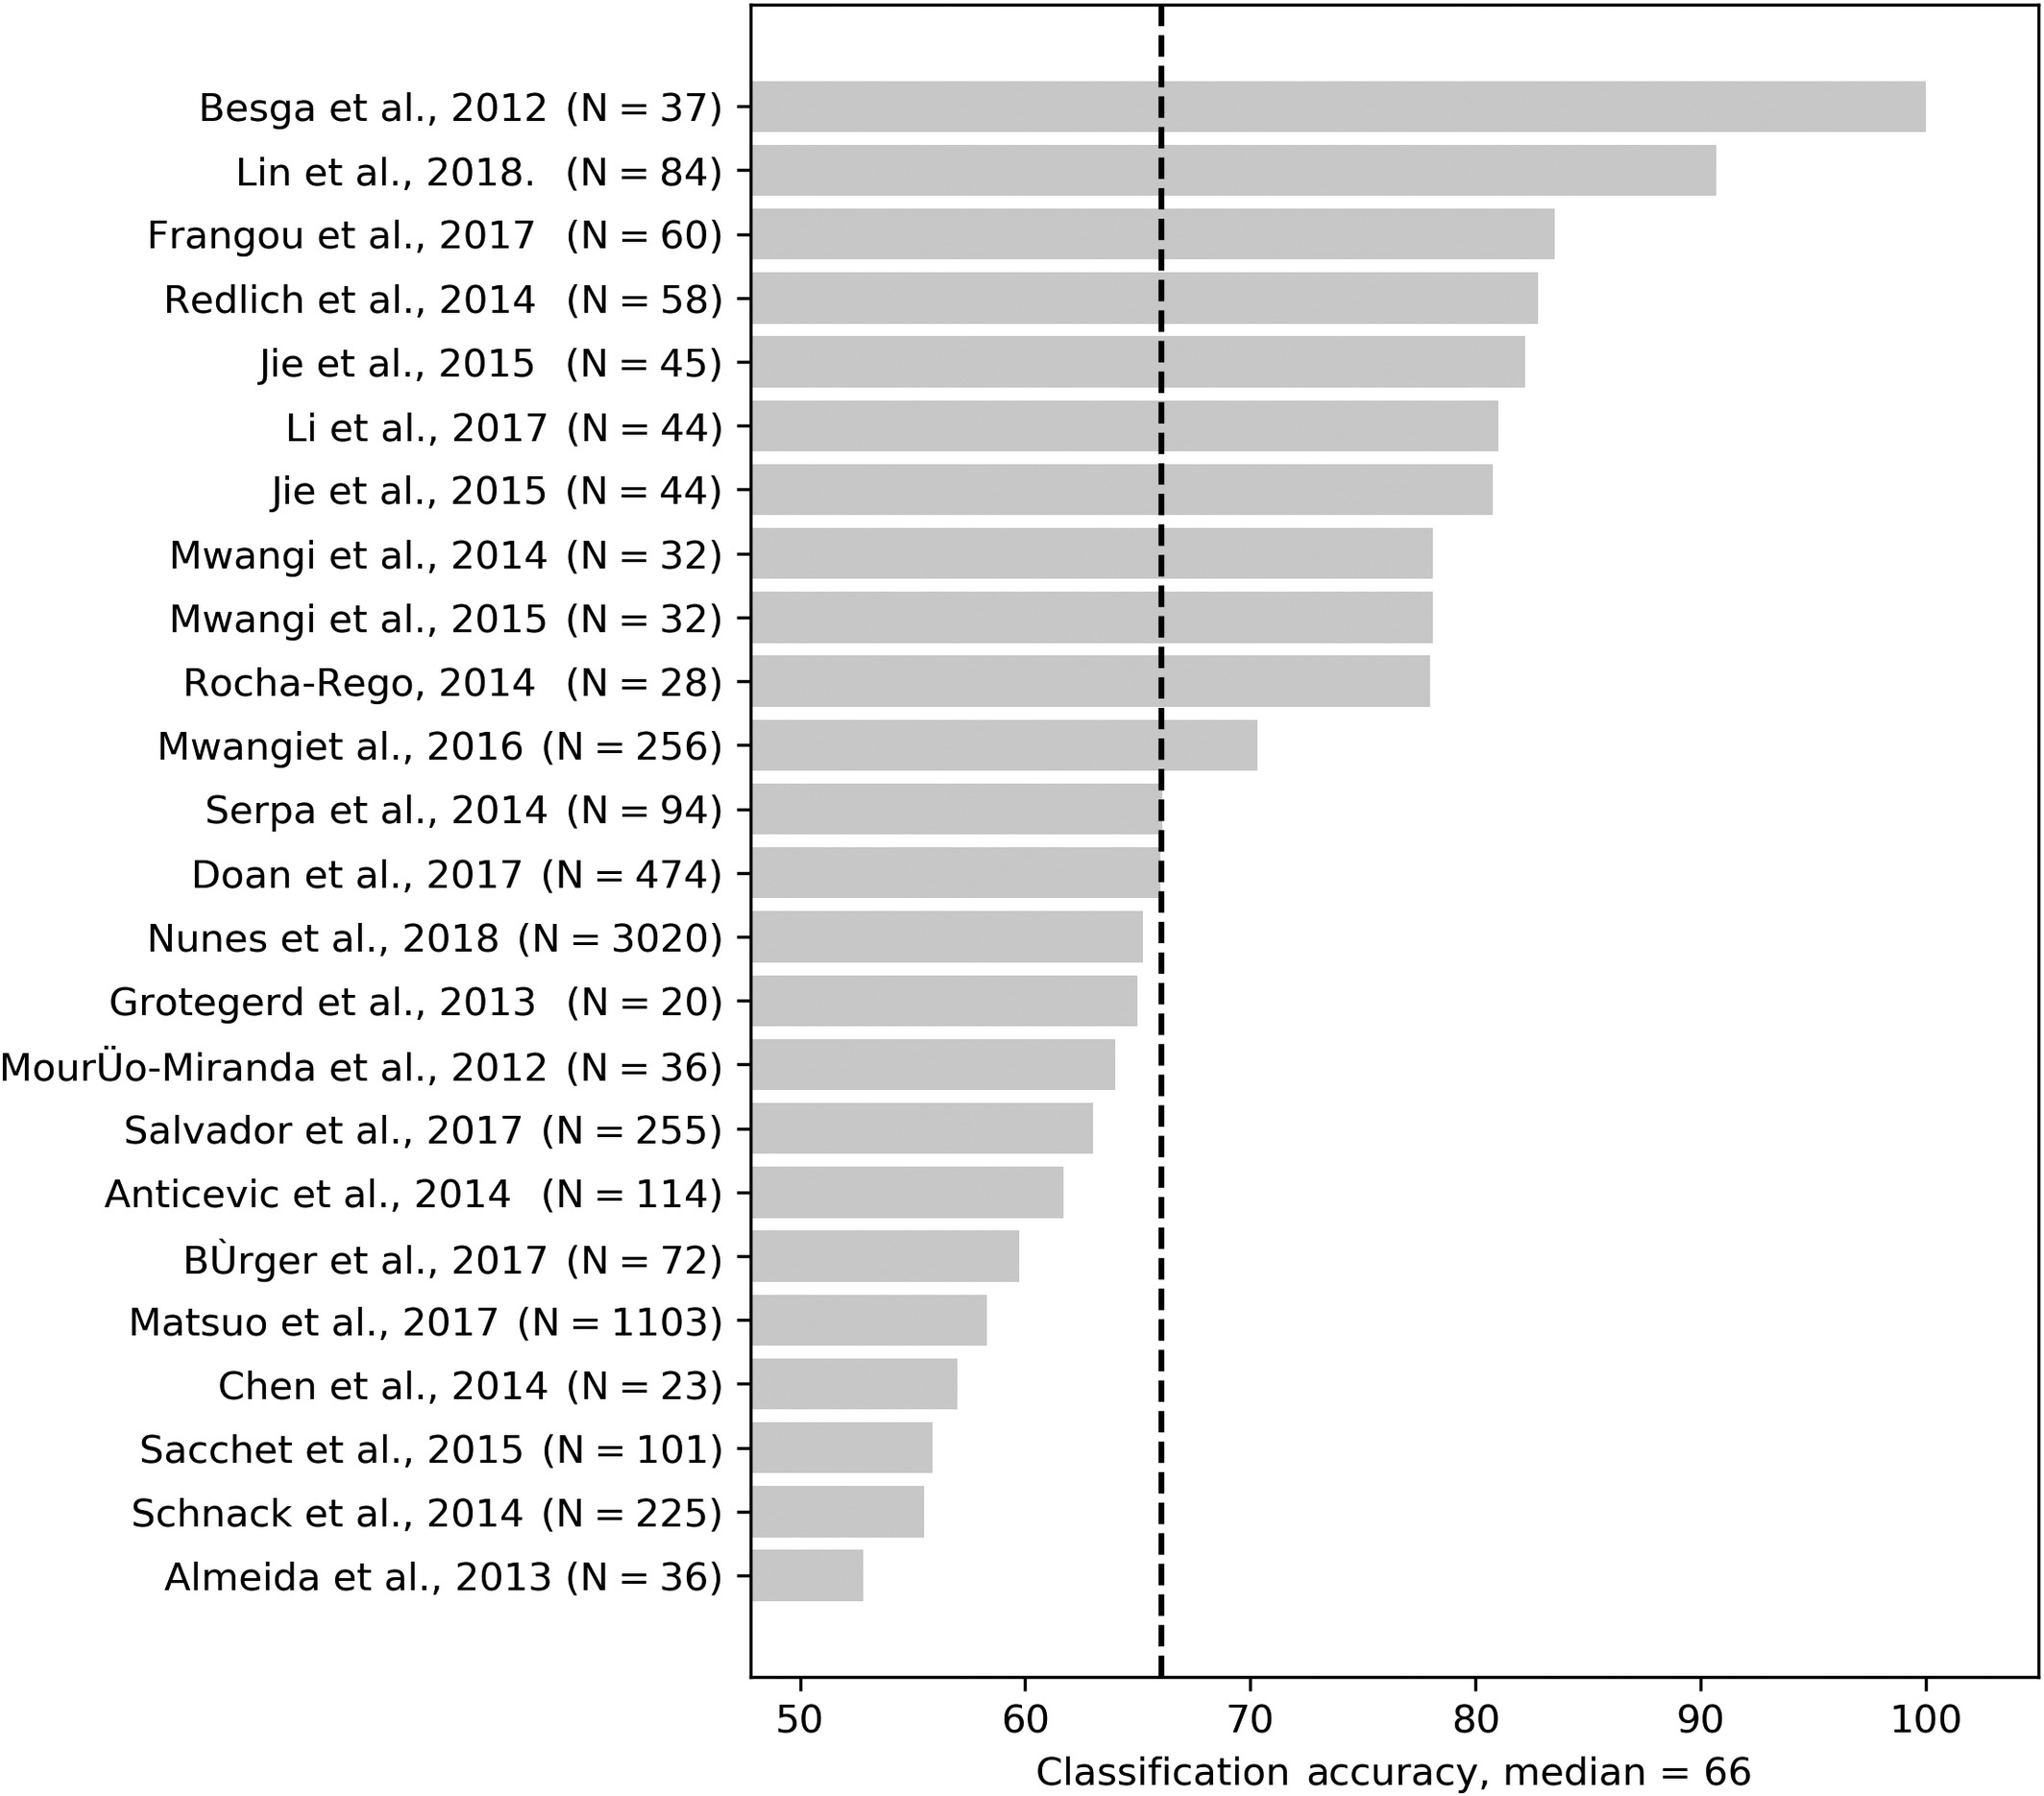
\includegraphics[width=8cm]{data/bp_accuracies.jpeg}
    %             };
    %         }
    %         \only<2>{
    %             % https://academic.oup.com/cercor/article/29/1/202/4653730?login=false
    %             \node[inner sep=0pt, draw=black] at (0, 0) {
    %                 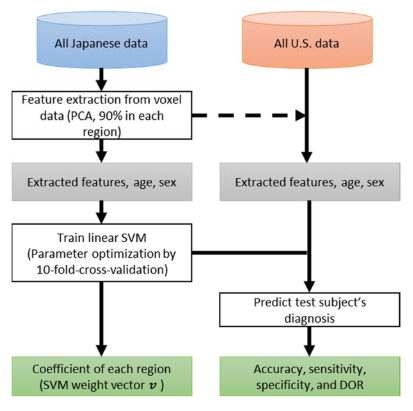
\includegraphics[width=6cm]{data/bp_generalization.png}
    %             };
    %         }
    %     \end{tikzpicture}
    % \end{frame}

    % \begin{frame}{Schizophrenia}
    % \end{frame}

    % \begin{frame}{Major depressive disorder}
    % \end{frame}

    % \section{The future of neuroimaging-based prediction}

    \newsavebox{\boxplots}
    \sbox{\boxplots}{%
    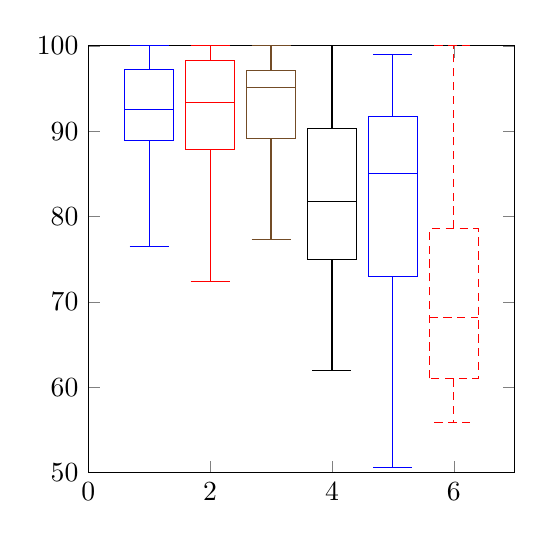
\begin{tikzpicture}
        \begin{axis}[
            boxplot/draw direction = y,
            width=7cm,
            height=7cm,
            xmin=0,
            xmax=7,
            ymin=50,
            ymax=100
        ]
        % DEM
        \addplot+[
            boxplot prepared={
              median=92.5,
              upper quartile=97.25,
              lower quartile=88.94,
              upper whisker=100,
              lower whisker=76.46
            },
        ] coordinates {};

        % MS
        \addplot+[
            boxplot prepared={
              median=93.4,
              upper quartile=98.26,
              lower quartile=87.9,
              upper whisker=100,
              lower whisker=72.36
            },
        ] coordinates {};

        % PD
        \addplot+[
            boxplot prepared={
              median=95.15,
              upper quartile=97.07,
              lower quartile=89.15,
              upper whisker=100,
              lower whisker=77.26
            },
        ] coordinates {};

        % SCZ
        \addplot+[
            boxplot prepared={
              median=81.8,
              upper quartile=90.28,
              lower quartile=75,
              upper whisker=100,
              lower whisker=62
            },
        ] coordinates {};

        % MDD
        \addplot+[
            boxplot prepared={
              median=85,
              upper quartile=91.7,
              lower quartile=73,
              upper whisker=99,
              lower whisker=50.55
            },
        ] coordinates {};

        % BP
        \addplot+[
            boxplot prepared={
              median=68.2,
              upper quartile=78.59,
              lower quartile=61.03,
              upper whisker=100,
              lower whisker=55.9
            },
        ] coordinates {};
        \end{axis}
    \end{tikzpicture}
    }

    \begin{frame}{Challenges: Predictiveness}
        \begin{tikzpicture}
            \node[draw=black] at (0, 0) {};
            \node[draw=black] at (10, -7) {};

            \only<2>{
                \node[] at (5, -3.5) {
                    \usebox{\boxplots}
                };
            }
        \end{tikzpicture}
    \end{frame}

    \begin{frame}{Challenges: Diagnostic targets}
    \end{frame}

    \begin{frame}{Challenges: Interpretability}
    \end{frame}

    \begin{frame}
        \begin{tikzpicture}
            %https://doi.org/10.1007/s40708-015-0019-x
            \node[inner sep=0pt, draw=black] at (0, 0) {
                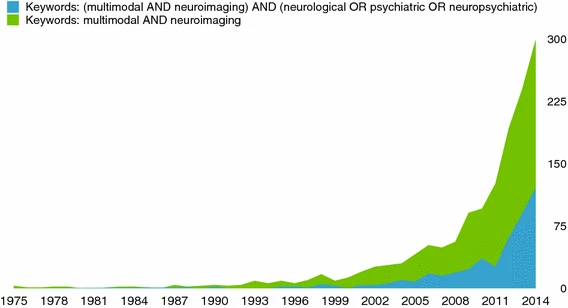
\includegraphics[width=4cm]{data/multimodal_progress.png}
            };
        \end{tikzpicture}
    \end{frame}
    \begin{frame}{The role of prediction}
        \centering
        \begin{tikzpicture}
            %https://doi.org/10.1038/s41380-022-01635-2
            \node[inner sep=0pt, draw=black] at (0, 0) {
                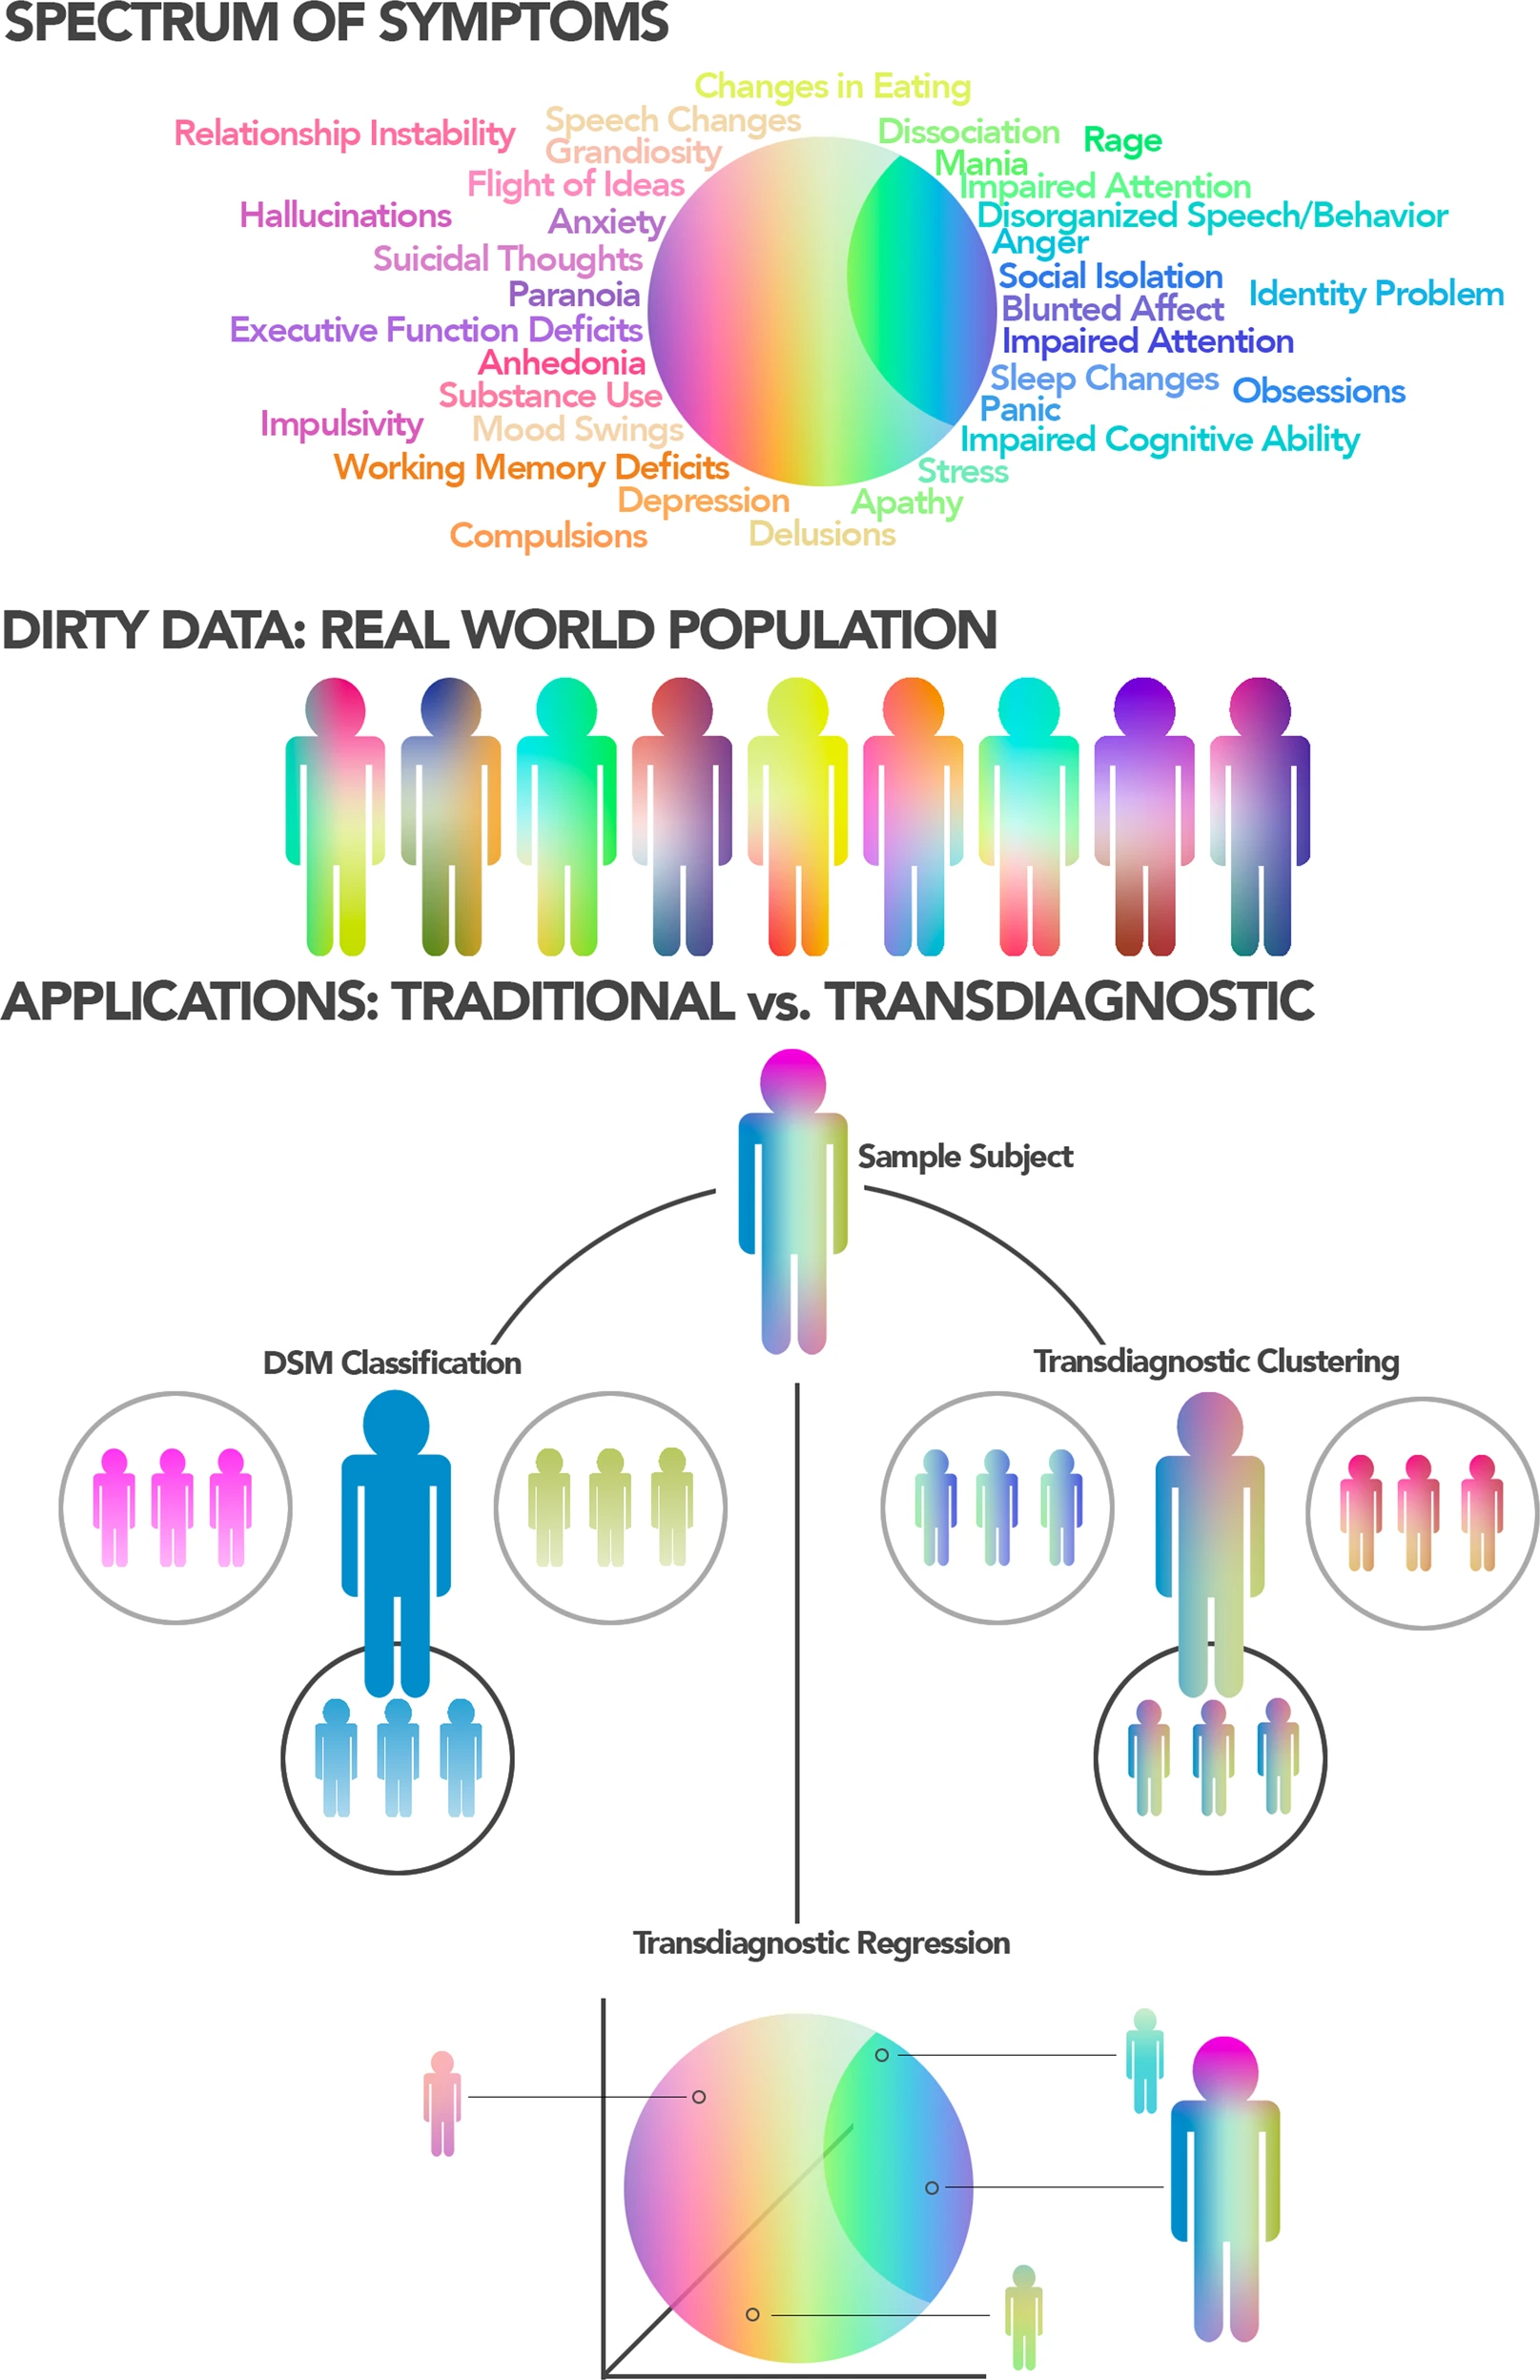
\includegraphics[width=4cm]{data/transdiagnostic.png}
            };
        \end{tikzpicture}
    \end{frame}


    \begin{frame}{Prediction versus interpretability}
        \centering
        \begin{tikzpicture}
            %https://doi.org/10.1038/s41380-022-01635-2
            \node[inner sep=0pt, draw=black] at (0, 0) {
                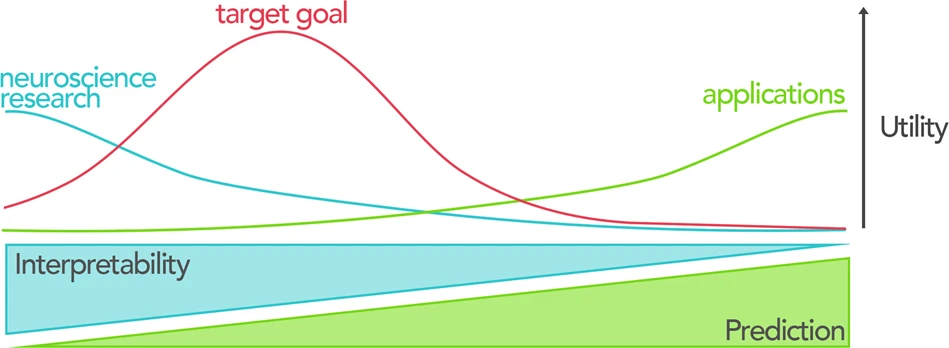
\includegraphics[width=8cm]{data/prediction_vs_interpretability.png}
            };
        \end{tikzpicture}
    \end{frame}
\end{document}
